\documentclass[tikz,border=3mm]{standalone}
\usepackage{tikz}
\usetikzlibrary{shapes,arrows,positioning,fit,backgrounds,calc}
\begin{document}
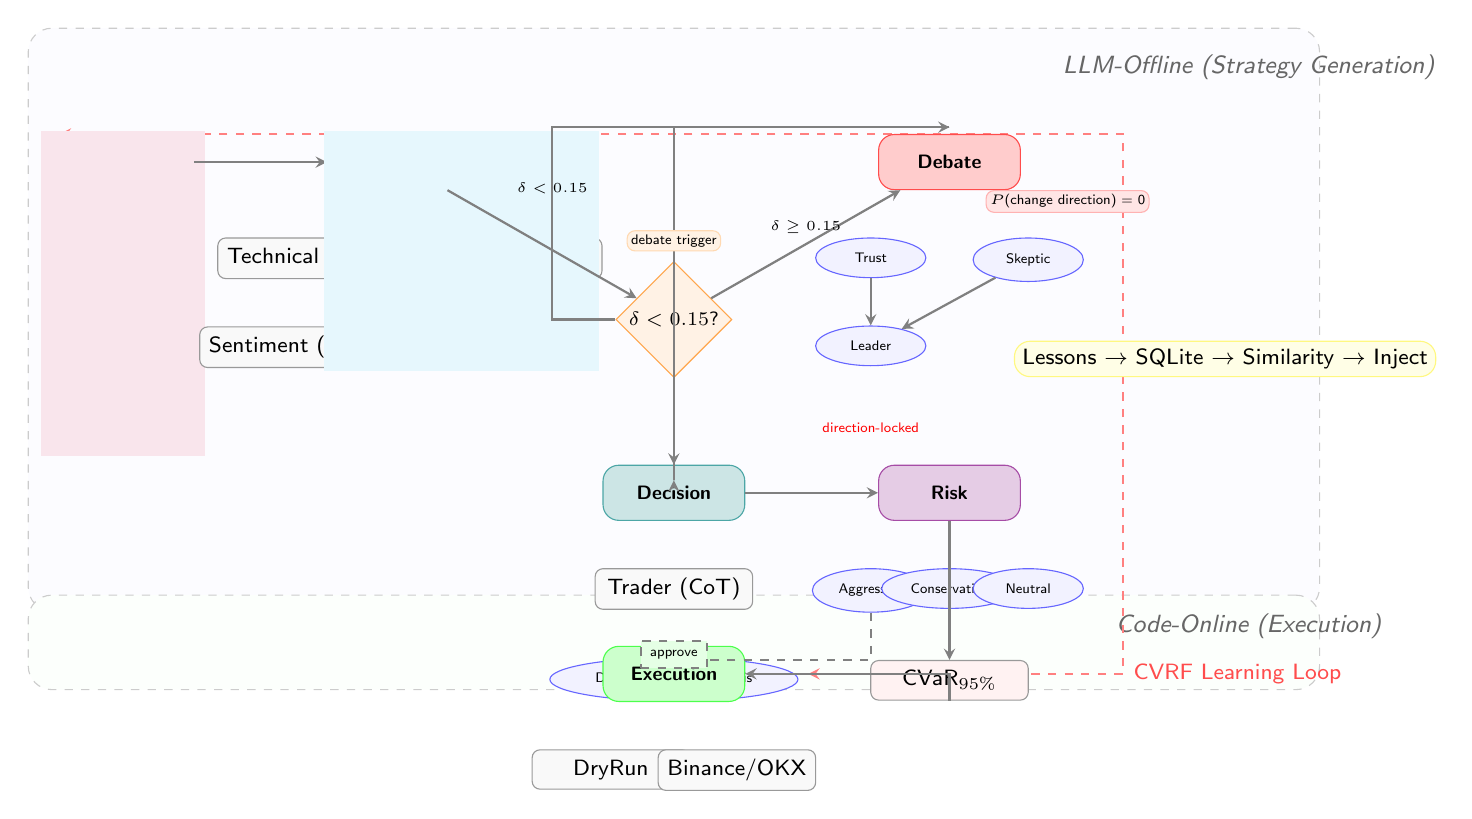
\begin{tikzpicture}[
  node distance=6mm and 12mm,
  stage/.style={rectangle, draw=#1!70, fill=#1!20, rounded corners=2mm,
    minimum width=18mm, minimum height=7mm, font=\sffamily\scriptsize\bfseries},
  agent/.style={rectangle, draw=black!40, fill=gray!5, rounded corners=1mm,
    minimum width=20mm, minimum height=5mm, font=\sffamily\footnotesize},
  role/.style={ellipse, draw=blue!60, fill=blue!5, minimum width=14mm,
    minimum height=4mm, font=\sffamily\tiny},
  arrow/.style={->,>=stealth,thick,draw=black!50},
  darrow/.style={<->,>=stealth,thick,draw=red!50,dashed},
  box/.style={rectangle, draw=black!20, rounded corners=3mm, dashed,
    inner sep=2mm, fill=black!2},
  label/.style={font=\sffamily\small\itshape, text=black!60},
]

% ===== Background layers =====
\begin{scope}[on background layer]
  \node[box,fit={(0.5,0.5) (16.5,7.5)},fill=blue!1] {};
  \node[label] at (15.8,7.2) {LLM-Offline (Strategy Generation)};
  \node[box,fit={(0.5,-0.5) (16.5,0.3)},fill=green!1] {};
  \node[label] at (15.8,0.1) {Code-Online (Execution)};
\end{scope}

% ===== Stage 1: Data Collection =====
\node[stage=purple] (data) at (1.5,6) {Data};
\node[agent,below=of data] (klines) {Klines};
\node[agent,below=of klines] (ob) {Orderbook};
\node[agent,below=of ob] (news) {News};

\node[fill=purple!10,inner sep=1pt,fit={(data) (news)},label={[purple]90:Stage 1}] {};

% ===== Stage 2: Analysis =====
\node[stage=cyan] (analysis) at (5,6) {Analysis};
\node[agent,below=of analysis,xshift=-10mm] (tech) {Technical (Claude)};
\node[agent,below=of analysis,xshift=10mm] (fund) {Fundamental (GPT-4o)};
\node[agent,below=of tech] (sent) {Sentiment (DeepSeek)};
\node[agent,below=of fund] (macro) {Macro/News (Claude)};

\draw[arrow] (data) -- (analysis);
\node[fill=cyan!10,inner sep=1pt,fit={(analysis) (macro)},label={[cyan]90:Stage 2}] {};

% ===== Disagreement =====
\node[diamond,draw=orange!70,fill=orange!10,inner sep=1pt,
  font=\sffamily\scriptsize,minimum size=10mm] (delta) at (8.5,4)
  {$\delta < 0.15$?};

\draw[arrow] (analysis) -- (delta);

% ===== Stage 3: Debate =====
\node[stage=red] (debate) at (12,6) {Debate};
\node[role,below=of debate,xshift=-10mm] (trust) {Trust};
\node[role,below=of debate,xshift=10mm] (skeptic) {Skeptic};
\node[role,below=of trust] (leader) {Leader};
\draw[arrow] (trust) -- (leader);
\draw[arrow] (skeptic) -- (leader);
\node[below=of leader,font=\sffamily\tiny,text=red] {direction-locked};

\draw[arrow] (delta) -- node[above,font=\sffamily\tiny] {$\delta \ge 0.15$} (debate);
\draw[arrow] (delta.west) -- ++(-0.8,0) |- ([yshift=8mm] debate.south)
  node[pos=0.3,above,font=\sffamily\tiny] {$\delta < 0.15$};

% ===== Stage 4: Decision =====
\node[stage=teal] (decision) at (8.5,1.8) {Decision};
\node[agent,below=of decision] (trader) {Trader (CoT)};
\node[role,below=of trader,font=\sffamily\tiny] (cot) {Data$\rightarrow$Concept$\rightarrow$Thesis};
\draw[arrow] ([yshift=8mm]debate.south) -| (decision);

% ===== Stage 5: Risk =====
\node[stage=violet] (risk) at (12,1.8) {Risk};
\node[role,below=of risk,xshift=-10mm] (aggr) {Aggressive};
\node[role,below=of risk] (cons) {Conservative};
\node[role,below=of risk,xshift=10mm] (neut) {Neutral};
\node[below=of cons,font=\sffamily\tiny,text=violet] {any-veto $\rightarrow$ reject};

\draw[arrow] (decision) -- (risk);
\draw[arrow] (delta.south) |- ([yshift=-2mm] decision.north);

% ===== CVaR =====
\node[agent,below=of aggr,xshift=10mm,fill=red!5] (cvar) {CVaR$_{95\%}$};
\draw[arrow] (risk) -- (cvar);

% ===== Execution =====
\node[stage=green] (exec) at (8.5,-0.5) {Execution};
\draw[arrow] (cvar.south) |- (exec);

\node[agent,below=of exec,xshift=-8mm] (dryrun) {DryRun};
\node[agent,below=of exec,xshift=8mm] (live) {Binance/OKX};
\draw[arrow,dashed] (aggr.south) -- ++(0,-0.6) -| (exec) node[pos=0.7,font=\sffamily\tiny,draw,fill=green!10] {approve};

% ===== CVRF Loop =====
\begin{scope}[on background layer]
  \draw[darrow,thick] ([xshift=8mm]exec.east) -- ++(4,0)
    node[right,font=\sffamily\footnotesize,text=red!70] {CVRF Learning Loop}
    |- ([xshift=-8mm]data.north);
\end{scope}

\node[fill=yellow!10,draw=yellow!50,rounded corners=2mm,inner sep=1mm,
  font=\sffamily\footnotesize] at (15.5,3.5)
  {Lessons $\rightarrow$ SQLite $\rightarrow$ Similarity $\rightarrow$ Inject};

% ===== Annotations =====
\node[fill=red!10,draw=red!30,rounded corners=1mm,inner sep=0.5mm,
  font=\sffamily\tiny] at (13.5,5.5) {$\mathbb{P}$(change direction) = 0};

\node[fill=orange!10,draw=orange!30,rounded corners=1mm,inner sep=0.5mm,
  font=\sffamily\tiny] at (8.5,5) {debate trigger};

\end{tikzpicture}
\end{document}
